%! Author = itgramic
%! Date = 29.12.23

% Preamble
\begin{flushleft}
    \subsubsection{Kosten-Nutzen}
    Patroni, in seinen beiden Ausprägungen als normales Patroni und mit dem \texttt{postgresql\_cluster}-Ansible \Gls{GitHub}-Repository\\
    ist klar die beste Variante:
    \begin{figure}[H]
        \centering
        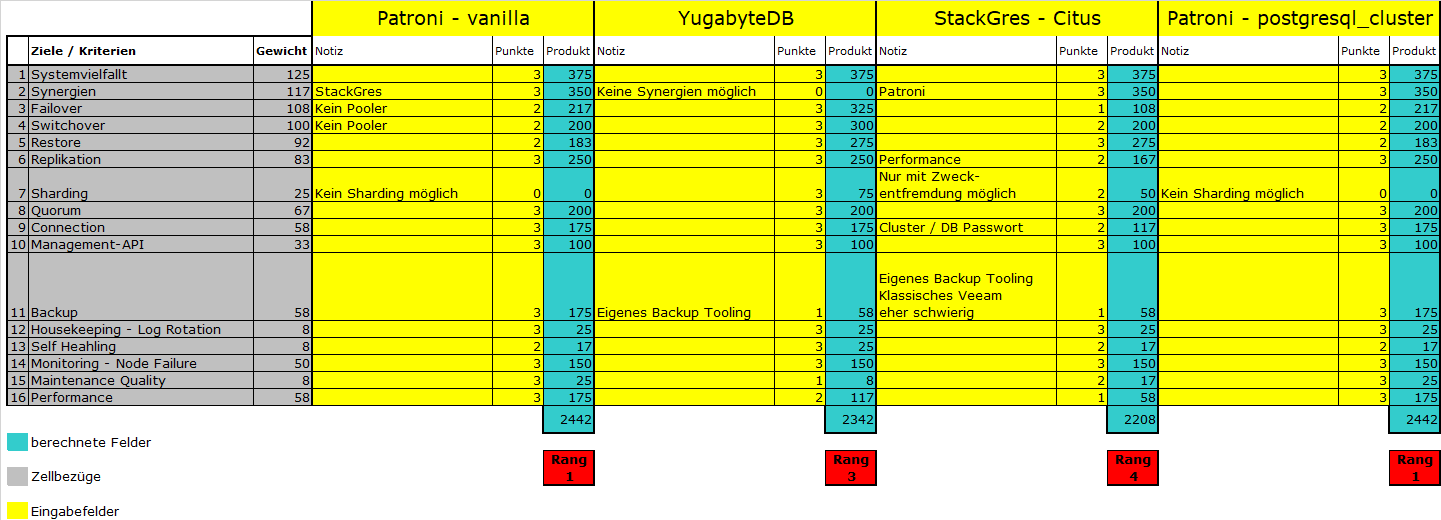
\includegraphics[width=1\linewidth]{source/implementation/evaluation/solution_comparison/nutzwert_analyse}
        \caption{Kosten-Nutzen-Analyse}
        \label{fig:nutzwert_analyse}
    \end{figure}
\end{flushleft}
\begin{flushleft}
    Bei den Kosten zeigt sich, dass die Patroni-Variante \texttt{postgresql\_cluster} klar am günstigsten kommt.\\
    Dies resultiert auf den tiefen Installationskosten und der schnellen Erweiterungen.
\end{flushleft}
\begin{flushleft}
    Da, dass Repository schon einiges an Ansible-Playbooks mitbringt, ist auch der Erweiterungsaufwand gering.\\
    YugabyteDB liegt auf Platz zwei, gefolgt vom klassischen (Vanilla) Patroni.
\end{flushleft}
\begin{flushleft}
    Auf dem letzten Platz landet StackGres - Citus, dies weil die Erstellung eines Clusters sehr viel Zeit benötigt.
    \begin{figure}[H]
        \centering
        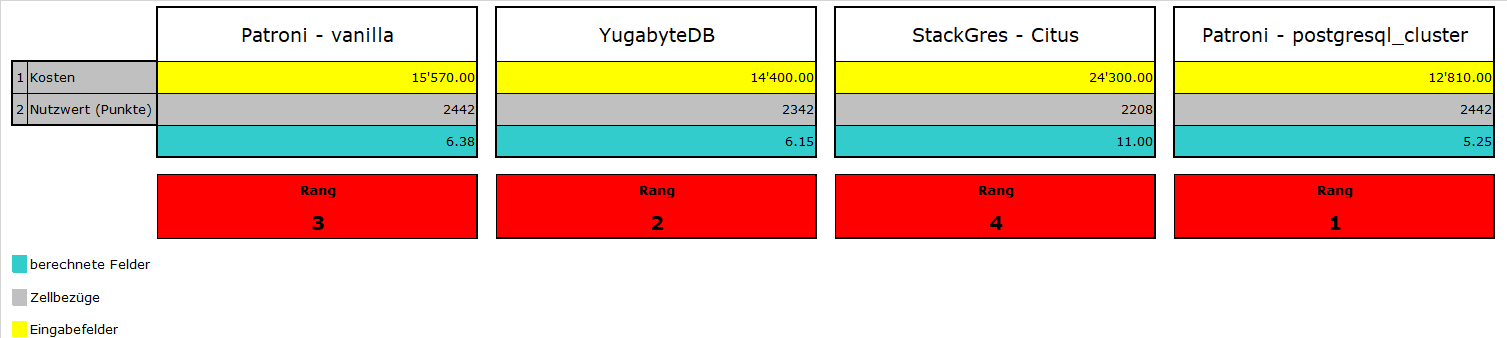
\includegraphics[width=1\linewidth]{source/implementation/evaluation/solution_comparison/cost_benefit_ranking}
        \caption{Kosten-Nutzen-Ranking}
        \label{fig:cost_benefit_ranking}
    \end{figure}
\end{flushleft}
\begin{flushleft}
    Daraus ergibt sich folgendes Kosten-Nutzen-Diagramm:
    \begin{figure}[H]
        \centering
        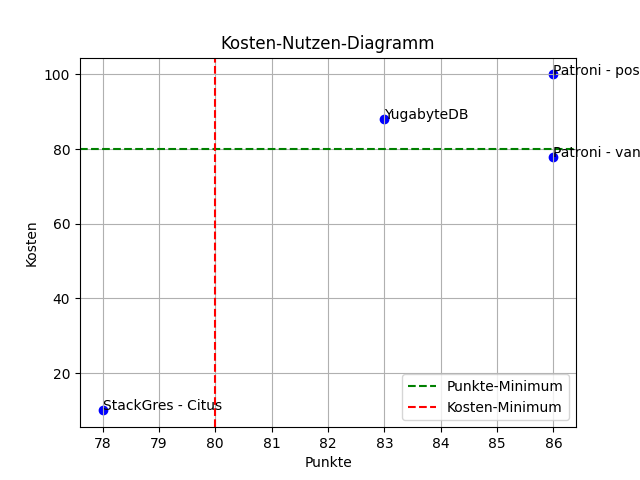
\includegraphics[width=1\linewidth]{source/cost_benefit_diagram/cost_benefit_diagram}
        \caption{Kosten-Nutzen-Diagramm}
        \label{fig:cost_benefit_diagram}
    \end{figure}
    StackGres - Citus scheidet direkt aus, da es nur 77\% der geforderten Punktezahl erreicht.\\
    Aber auch das klassische Patroni scheidet aus,\\
    dies, weil die Kosten im Verhältnis zur besten Variante (\texttt{postgresql\_cluster}) ebenfalls unter der 80\% Marke liegt.
\end{flushleft}